\label{sec:classification}
Nachdem in vorherigen Abschnitt eine passende Merkmalsmenge erstellt wurde, geht es nun um die Entscheidung, ob der Fahrer Müde oder Wach ist bzw. ob das System eine Müdigkeitsmeldung erscheinen lässt. Für diese Klassifizierung werden im allgemeinen Machine-Learning-Algorithmen verwendet. Anhand von markierten Datensätzen wird versucht den Algorithmus zu Trainieren (Überwachtes Lernen). Dies dient dem Ziel, dass er auch unbekannte Daten klassifizieren kann. Dieser Vorgang wird Generalisierung bezeichnet und ist auch im menschlichen Lernen ein wichtiger Schritt.

Für die Anwendung wurde zur Klassifizierung ein künstliches Neuronales Netz  ausgewählt. Es basiert auf einem erweiterten McCulloch-Pitts-Neuron \cite{ann} und ist der Funktionsweise des menschlichen Gehirns bzw. seinen Neuronen nachempfunden\cite{marsland_opac-b1129336}. Ein KNN lässt sich im einfachste Fall durch eine Merkmalsmenge $X = x_1, x_2 ... x_n$, dazugehörige Gewichte $W = w_1, w_2 ... w_n$, eine Übertragungsfunktion $\sum$ und eine Schwellwertfunktion $\theta$ beschreiben (Abb. \ref{fig:perceptron}).

\begin{figure}[h] 
  \begin{center}
    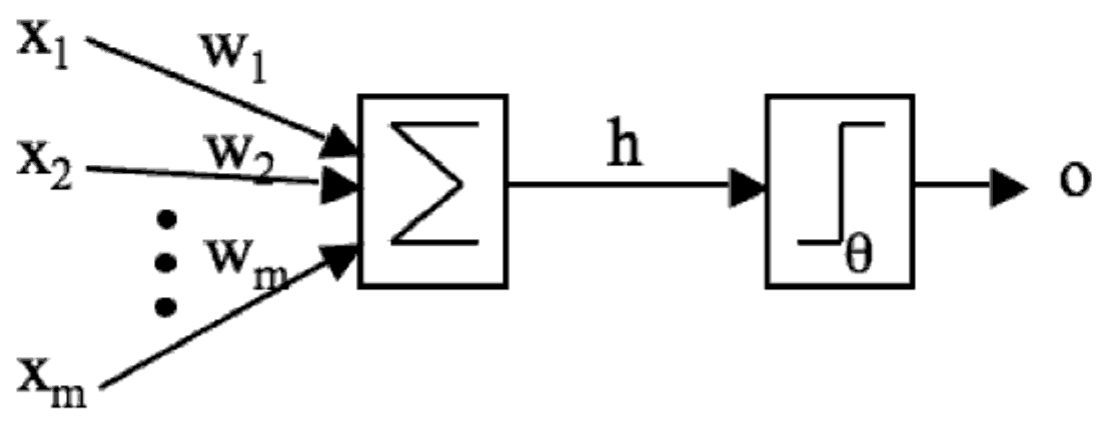
\includegraphics[width=5.5cm]{perceptron}
    \caption[Perceptron]{Darstellung eines McCulloch-Pitts-Neurons. Die Merkmale $X$ werden mit den Gewichten $W$ multiplziert und in $\sum$ summiert. Wenn $h > \theta$ "`feuert"' das Neuron ($o = 1$) \cite{marsland_opac-b1129336}. \label{fig:perceptron}}
  \end{center}
\end{figure}

Dieser vereinfachte Aufbau kann schon einfach Aufgaben, wie bspw. ein logisches "`UND"', erfüllen. Schon ein logisches "`XOR"' lässt sich nicht mehr abbilden. Dafür muss eine oder mehrere Schichten von Neuronen (Hidden Layers) hintereinander geschaltet werden (Abb. \ref{fig:mlp}).

\begin{figure}[h] 
  \begin{center}
    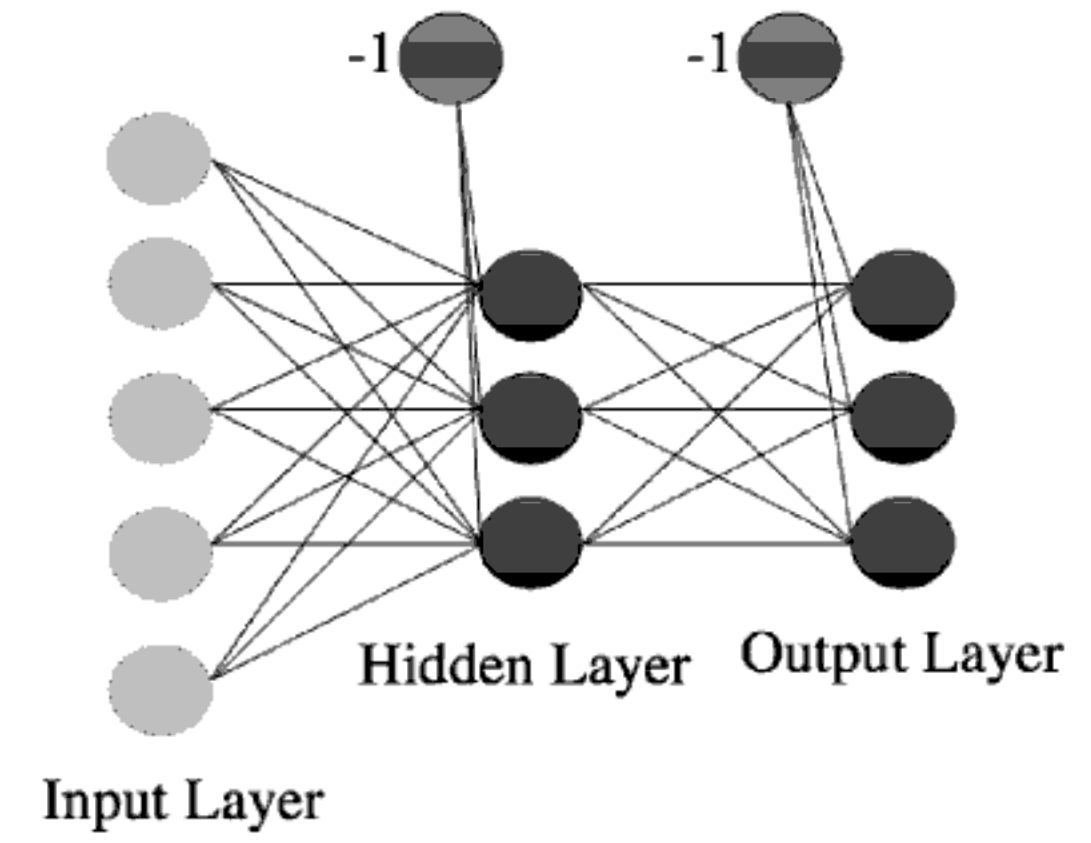
\includegraphics[width=5.5cm]{mlp}
    \caption[MLP]{Darstellung eines Neuronalen Netzes mit mehreren Schichten (Multi Layer Perceptron, MLP)\cite{marsland_opac-b1129336}. \label{fig:mlp}}
  \end{center}
\end{figure}

\textbf{TODO}